\documentclass{article}

\usepackage[utf8]{inputenc}
\usepackage{amsmath}
\usepackage{amssymb}
\usepackage{amsthm}
\usepackage{ifthen}
\usepackage{xparse}
%\usepackage{tikz}
%\usetikzlibrary{decorations.fractals}
\usepackage{graphicx}

\newcommand{\sizedescriptor}[2]
{
\ifthenelse{\equal{#1}{0}}{}{
\ifthenelse{\equal{#1}{1}}{\big}{
\ifthenelse{\equal{#1}{2}}{\Big}{
\ifthenelse{\equal{#1}{3}}{\bigg}{
\ifthenelse{\equal{#1}{4}}{\Bigg}{
#2}}}}}
}

\NewDocumentCommand{\set}
{O{auto} m G{\empty}}
{\sizedescriptor{#1}{\left}\{ {#2} \ifthenelse{\equal{#3}{}}{}{ \; \sizedescriptor{#1}{\middle}| \; {#3}} \sizedescriptor{#1}{\right}\}}

\newcommand{\pow}{\mathcal{P}}

\newcommand{\all}[1]{\forall #1 .\,}
\newcommand{\some}[1]{\exists #1 .\,}
\newcommand{\exactlyone}[1]{\exists{!} #1 .\,}
\newcommand{\lam}[1]{\lambda #1 .\,}
\newcommand{\that}[1]{\iota #1 .\,}

\usepackage[slovene]{babel}
\newcommand{\lthen}{\Rightarrow}
\newcommand{\two}{\mathbf{2}}
\newcommand{\true}{\top}
\newcommand{\false}{\bot}

\newcommand{\NN}{\mathbb{N}}
\newcommand{\ZZ}{\mathbb{Z}}
\newcommand{\QQ}{\mathbb{Q}}
\newcommand{\RR}{\mathbb{R}}

%%%%%%%%%%%%%%%%%%%%%%%%%%%%%%%%%%%%%%%%%%%%%%%%%%%%%%%%%%%%%%%%%%%%%%%%%%%%%%%%%%%%%%%%%%%%%%%%%%%%%%%%%%%%%%%%%%%%%%%
%%%  Commands
%%%%%%%%%%%%%%%%%%%%%%%%%%%%%%%%%%%%%%%%%%%%%%%%%%%%%%%%%%%%%%%%%%%%%%%%%%%%%%%%%%%%%%%%%%%%%%%%%%%%%%%%%%%%%%%%%%%%%%


%%%%%%%%%%%%%%%%%%%%%%%%%%%%%%%%%%%%%%%%%%%%%%%%%%%%%%%%%%%%%
%%%  Theorems etc.
%%%%%%%%%%%%%%%%%%%%%%%%%%%%%%%%%%%%%%%%%%%%%%%%%%%%%%%%%%%%%
{
\theoremstyle{theorem}
\newtheorem{izrek}{Izrek}[chapter]
\newtheorem{lema}[izrek]{Lema}
\newtheorem{trditev}[izrek]{Trditev}
\newtheorem{posledica}[izrek]{Posledica}
\newtheorem{pravilo}[izrek]{Pravilo}
}

{
\theoremstyle{definition}
\newtheorem{definicija}[izrek]{Definicija}
\newtheorem{opomba}[izrek]{Opomba}
\newtheorem{primer}[izrek]{Primer}
\newtheorem{zgled}[izrek]{Zgled}
\newtheorem{naloga}[izrek]{Naloga}
}


%%%%%%  Proofs
%%%%%%%%%%%%%%%%%%%%%%%%%%%%%%%%%%%%%%%%%%%%%%%%%%%%%%%%%%%%%
% Za dokaze uporabimo amsmath proof, sicer ne deluje \qedhere.


%%%%%%  Auxiliary
%%%%%%%%%%%%%%%%%%%%%%%%%%%%%%%%%%%%%%%%%%%%%%%%%%%%%%%%%%%%%
\newcommand{\sizedescriptor}[2]
{
\ifthenelse{\equal{#1}{0}}{}{
\ifthenelse{\equal{#1}{1}}{\big}{
\ifthenelse{\equal{#1}{2}}{\Big}{
\ifthenelse{\equal{#1}{3}}{\bigg}{
\ifthenelse{\equal{#1}{4}}{\Bigg}{
#2}}}}}
}

\newcommand{\someref}{{\small\textcolor{blue}{[\textbf{ref.}]}}}
\newcommand{\intermission}{\bigskip\medskip}
\newcommand{\ltc}[1]{$\backslash$\texttt{#1}}  % LaTeX command
\newcommand{\nls}[1]{``\textit{#1}''}  % sentence in a natural language

%%%%%%  Logical Quantifiers, λ- and ι-Expressions
%%%%%%%%%%%%%%%%%%%%%%%%%%%%%%%%%%%%%%%%%%%%%%%%%%%%%%%%%%%%%

\newcommand{\all}[1]{\forall #1 .\,}
\newcommand{\some}[1]{\exists #1 .\,}
\newcommand{\exactlyone}[1]{\exists{!} #1 .\,}
\newcommand{\lam}[1]{\lambda #1 .\,}
\newcommand{\that}[1]{\iota #1 .\,}

%%%%%%  Logic
%%%%%%%%%%%%%%%%%%%%%%%%%%%%%%%%%%%%%%%%%%%%%%%%%%%%%%%%%%%%%
\newcommand{\tvs}{\Omega}  % set of truth values
\newcommand{\true}{\top}  % truth
\newcommand{\false}{\bot}  % falsehood
\newcommand{\etrue}{\boldsymbol{\top}}  % emphasized truth
\newcommand{\efalse}{\boldsymbol{\bot}}  % emphasized falsehood
\newcommand{\impl}{\Rightarrow}  % implication sign
\newcommand{\revimpl}{\Leftarrow}  % reverse implication sign
\newcommand{\lequ}{\Leftrightarrow}  % equivalence sign
\newcommand{\xor}{\mathbin{\veebar}}  % exclusive disjunction sign
\newcommand{\shf}{\mathbin{\uparrow}}  % Sheffer connective
\newcommand{\luk}{\mathbin{\downarrow}}  % Łukasiewicz connective


%%%%%%  Sets
%%%%%%%%%%%%%%%%%%%%%%%%%%%%%%%%%%%%%%%%%%%%%%%%%%%%%%%%%%%%%
%  \set{1, 2, 3}         ->  {1, 2, 3}
%  \set{a \in X}{a < 1}  ->  {a ∈ X | a < 1}
\NewDocumentCommand{\set}
{O{auto} m G{\empty}}
{\sizedescriptor{#1}{\left}\{ {#2} \ifthenelse{\equal{#3}{}}{}{ \; \sizedescriptor{#1}{\middle}| \; {#3}} \sizedescriptor{#1}{\right}\}}
%\newcommand{\vsubset}{\Mapstochar\cap}
%\newcommand{\finseq}[1]{{#1}^*}
\newcommand{\pst}{\mathcal{P}}
\renewcommand{\complement}[1]{{#1}^C}


%%%%%%  Number Sets, Intervals
%%%%%%%%%%%%%%%%%%%%%%%%%%%%%%%%%%%%%%%%%%%%%%%%%%%%%%%%%%%%%
\newcommand{\NN}{\mathbb{N}}
\newcommand{\ZZ}{\mathbb{Z}}
\newcommand{\QQ}{\mathbb{Q}}
\newcommand{\RR}{\mathbb{R}}
\newcommand{\CC}{\mathbb{C}}
\newcommand{\intoo}[3][\RR]{{#1}_{(#2, #3)}}
\newcommand{\intcc}[3][\RR]{{#1}_{[#2, #3]}}
\newcommand{\intoc}[3][\RR]{{#1}_{(#2, #3]}}
\newcommand{\intco}[3][\RR]{{#1}_{[#2, #3)}}


%%%%%%  Maps and Relations
%%%%%%%%%%%%%%%%%%%%%%%%%%%%%%%%%%%%%%%%%%%%%%%%%%%%%%%%%%%%%
\newcommand{\id}[1][]{\mathrm{id}_{#1}}  % identity map
\newcommand{\argbox}{{\;\!\fbox{\phantom{M}}\;\!}}  % box for a function argument
\newcommand{\konst}[1]{\mathrm{k}_{#1}} % constant map
\newcommand{\rstr}[1]{\left.{#1}\right|}  % map restriction
\newcommand{\im}{\mathrm{im}}  % map image
\newcommand{\parto}{\mathrel{\rightharpoonup}}  % partial mapping sign
\NewDocumentCommand{\rel}
{O{\empty} O{\empty}}
{\ifthenelse{\equal{#1}{}}{\mathscr{R}}{{#1} \mathrel{\mathscr{R}} {#2}}}  % a relation
\NewDocumentCommand{\srel}
{O{\empty} O{\empty}}
{\ifthenelse{\equal{#1}{}}{\mathscr{S}}{{#1} \mathrel{\mathscr{S}} {#2}}}  % a second relation
\newcommand{\dom}{\mathrm{dom}}  % domain
\newcommand{\cod}{\mathrm{cod}}  % codomain
\newcommand{\dd}[1]{D_{#1}}  % domain of definition
\newcommand{\rn}[1]{Z_{#1}}  % range
\newcommand{\graph}[1]{\Gamma_{#1}}  % graph of a (partial) function
\NewDocumentCommand{\img}  % image
{O{\empty} m G{\empty}}
{{#2}_*\ifthenelse{\equal{#3}{}}{}{\!\sizedescriptor{#1}{\left}( {#3} \sizedescriptor{#1}{\right})}}
\NewDocumentCommand{\pim}  % preimage
{O{\empty} m G{\empty}}
{{#2}^*\ifthenelse{\equal{#3}{}}{}{\!\sizedescriptor{#1}{\left}( {#3} \sizedescriptor{#1}{\right})}}
\newcommand{\ec}[2][]{[\:\!{#2}\:\!]_{#1}}  % equivalence class
\newcommand{\transposed}[1]{\widehat{#1}}


%%%%%%  Projections and Injections
%%%%%%%%%%%%%%%%%%%%%%%%%%%%%%%%%%%%%%%%%%%%%%%%%%%%%%%%%%%%%
\NewDocumentCommand{\fst}
{O{\empty} O{\empty}}
{\pi_1^{{#1}\ifthenelse{\equal{#2}{}}{}{,}{#2}}}
\NewDocumentCommand{\snd}
{O{\empty} O{\empty}}
{\pi_2^{{#1}\ifthenelse{\equal{#2}{}}{}{,}{#2}}}
\NewDocumentCommand{\inl}
{O{\empty} O{\empty}}
{\iota_1^{{#1}\ifthenelse{\equal{#2}{}}{}{,}{#2}}}
\NewDocumentCommand{\inr}
{O{\empty} O{\empty}}
{\iota_2^{{#1}\ifthenelse{\equal{#2}{}}{}{,}{#2}}}


%%%%%%  Categories
%%%%%%%%%%%%%%%%%%%%%%%%%%%%%%%%%%%%%%%%%%%%%%%%%%%%%%%%%%%%%
\newcommand{\ct}[1]{\mathbf{#1}}
\newcommand{\mnoz}{\ct{Mno\check{z}}}
\newcommand{\pkol}{\ct{PKol}}  % category of semirings
\newcommand{\upkol}{\pkol_1}  % category of unital semirings
\newcommand{\kol}{\ct{Kol}}  % category of rings
\newcommand{\ukol}{\kol_1}  % category of unital rings


%%%%%%  Exercises and Solutions
%%%%%%%%%%%%%%%%%%%%%%%%%%%%%%%%%%%%%%%%%%%%%%%%%%%%%%%%%%%%%
\Newassociation{resitev}{Resitev}{resitve}
\renewcommand{\Resitevlabel}[1]{\emph{Re\v{s}itev~#1}}
{
\theoremstyle{definition}
\newtheorem{vaja}{Vaja}[chapter]
}


%%%%%%  Misc.
%%%%%%%%%%%%%%%%%%%%%%%%%%%%%%%%%%%%%%%%%%%%%%%%%%%%%%%%%%%%%
\renewcommand{\divides}{\,|\,}
% Načeloma bi morala biti navpična črta v \divides obdana z \mathrel, ampak to vodi do prevelikih presledkov.
\newcommand{\df}[1]{\emph{\textbf{#1}}}  % defined notion
\newcommand{\oper}{\mathop{\circledast}\nolimits}  % symbol for a generic operation
\newcommand{\soper}{\mathop{\boxasterisk}\nolimits}  % symbol for a second generic operation
\newcommand{\tconc}{\mathop{\bullet}\nolimits}  % symbol for binary tree concatenation
\newcommand{\ism}{\cong}  % isomorphic
\newcommand{\inv}[1]{#1^{-1}} % inverz preslikave
\newcommand{\equ}{\sim}  % equivalent
\newcommand{\dfeq}{\mathrel{\mathop:}=}  % definitional equality
\newcommand{\revdfeq}{=\mathrel{\mathop:}}  % reverse definitional equality
\newcommand{\isdefined}[1]{{#1}\!\downarrow}  % given value is defined
\newcommand{\kleq}{\simeq}  % Kleene equality
\newcommand{\claim}[3]{{#1} \;\colon\; \frac{#2}{#3}}  % claim, divided on context, assumptions, conclusions
\newcommand{\one}{\mathtt{\mathbf{1}}}  % generic singleton
\newcommand{\unit}{\mathord{()}}  % element in a generic singleton
\newcommand{\nul}{\mathtt{N}}  % null map
\newcommand{\suc}{\mathtt{S}}  % successor
\newcommand{\prd}{\mathtt{P}}  % predecessor
\newcommand{\tprd}{\tilde{\prd}}  % predecessor as a total function
\newcommand{\monus}{\mathbin{\vphantom{+}\text{\mathsurround=0pt \ooalign{\noalign{\kern-.35ex}\hidewidth$\smash{\cdot}$\hidewidth\cr\noalign{\kern.35ex}$-$\cr}}}}
% Definicija za monus pobrana s TeX Stack Exchange
\newcommand{\wf}{\prec}  % well-founded order
\NewDocumentEnvironment{implproof}  % proof of an implication
{O{\empty} G{\empty} O{=>} G{\empty}}
{
\begin{description}
\item[\quad$\sizedescriptor{#1}{\left}({#2}
\ifthenelse{\equal{#3}{=>}}{\impl}{
\ifthenelse{\equal{#3}{<=}}{\revimpl}{
\ifthenelse{\equal{#3}{->}}{\rightarrow}{
\ifthenelse{\equal{#3}{<-}}{\leftarrow}{
#3
}}}} {#4}\sizedescriptor{#1}{\right})$]\ \vspace{0.3em}\\
}
{
\end{description}
}


%%%%%%%%%%%%%%%%%%%%%%%%%%%%%%%%%%%%%%%%%%%%%%%%%%%%%%%%%%%%%%%%%%%%%%%%%%%%%%%%%%%%%%%%%%%%%%%%%%%%%%%%%%%%%%%%%%%%%%

%%% Local Variables:
%%% mode: latex
%%% TeX-master: "ucbenik-lmn"
%%% End:

{
\theoremstyle{definition}
\newtheorem{vaja}{Vaja}
}


\begin{document}

\title{Logika in množice -- vaje}
\date{22.~12.~2017}
\maketitle

\begin{vaja}
  Seštevanje na $\NN$ rekurzivno definiramo kot
  \begin{align*}
    &n + 0 := n, \\
    &n + m^+ := (n + m)^+.
  \end{align*}
  Dokažite naslednje trditve za vse $a, b, c \in \NN$ (pri tem $1 := 0^+$).
  \begin{enumerate}
    \item
      $a + 1 = a^+$
    \item
      $1 + a = a^+$
    \item
      $(a + b) + c = a + (b + c)$
    \item
      $a + b = b + a$
  \end{enumerate}
\end{vaja}

\begin{vaja}
	\emph{Končne nize} elementov iz množice $S$ označimo z $a_0 a_1 \ldots a_{n-1}$, kjer je $n \in \NN$ in $a_i \in S$ za $i \in \set{0, 1, 2, \ldots, n-1}$. \emph{Dolžina} $\ell$ končnega niza je število elementov v nizu, tj.~$\ell(a_0 a_1 \ldots a_{n-1}) = n$. Prazen niz označimo z $\varepsilon$ in velja $\ell(\varepsilon) = 0$.
	
	\emph{Stik} ali \emph{spoj} dveh končnih nizov dobimo tako, da za prvi niz pripnemo drugega. Stikanje označimo z dvojnim dvopičjem (::). Če sta torej $a_0 a_1 \ldots a_{n-1}$ in $b_0 b_1 \ldots b_{m-1}$ končna niza elementov iz množice $S$, potem je njun stik
	\[(a_0 a_1 \ldots a_{n-1}) :: (b_0 b_1 \ldots b_{m-1}) = a_0 a_1 \ldots a_{n-1} b_0 b_1 \ldots b_{m-1}.\]
	\begin{enumerate}
		\item
			Zgornje definicije niso povsem natančne, saj so podane s tropičji. Podajte induktivno definicijo končnih nizov in rekurzivni definiciji stika ter dolžine.
		\item
			Z indukcijo dokažite, da je dolžina staknjenega niza enaka vsoti dolžin ustreznih podnizov, tj.~če sta $a$ in $b$ končna niza, velja:
			\[\ell(a :: b) = \ell(a) + \ell(b).\]
	\end{enumerate}
\end{vaja}

\begin{vaja}
	Primer dvojiškega drevesa je na sliki \ref{fig:drevo}.
	\begin{figure}[!ht]
		\centering
		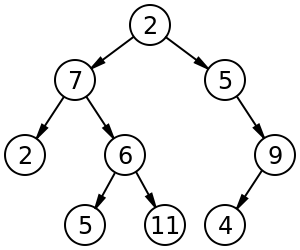
\includegraphics[width = 5cm]{Binary_tree.png}
		\caption{Primer dvojiškega drevesa.}
		\label{fig:drevo}
	\end{figure}
	
	\emph{Globina} drevesa je dolžina najdaljše poti od korena do (poljubnega) lista. Drevo na sliki ima globino $4$ (obstajajo tri različne poti, ki realizirajo to globino). Globina praznega drevesa je 0.  
	\emph{Obrnjeno drevo} dobimo iz dvojiškega drevesa, če vsakemu vozlišču zamenjamo levega in desnega otroka. 
	\begin{enumerate}
		\item Narišite obrnjeno drevo drevesa na sliki.
		\item Zapišite globino drevesa in obračanje drevesa kot rekurzivni funkciji na dvojiških drevesih.
		\item Z indukcijo dokažite, da je globina obrnjenega drevesa enaka globini prvotnega drevesa. 
	\end{enumerate}
\end{vaja}

\begin{vaja}
  Naj bo $A$ množica.
  \begin{enumerate}
    \item
      Dokažite: če je relacija $R \subseteq A \times A$ asimetrična, je irefleksivna.
    \item
      Dokažite: če je relacija $R \subseteq A \times A$ tranzitivna, sta zanjo asimetričnost in irefleksivnost ekvivalentni.
    \item
      Naj bo $\leq$ linearna ureditev na $A$. Dokažite, da je relacija $<$, definirana kot
      \[x < y \iff x \leq y \land x \neq y,\]
      stroga linearna ureditev na $A$ (to pomeni: $<$ je irefleksivna tranzitivna relacija, ki zadošča pogoju $\all{x, y \in A}{x \neq y \lthen x < y \lor y < x}$).
    \item
      Naj bo $<$ stroga linearna ureditev na $A$. Dokažite, da je relacija $\leq$, definirana kot
      \[x \leq y \iff x < y \lor x = y,\]
      linearna ureditev na $A$.
    \item
      Naj bo $\mathcal{L}_A$ množica linearnih ureditev na $A$ in $\mathcal{SL}_A$ množica strogih linearnih ureditev na $A$. Dokažite $\mathcal{L}_A \cong \mathcal{SL}_A$.
  \end{enumerate}
\end{vaja}

\begin{vaja}
  Konstruirajte dobro urejenost na množici racionalnih števil.
\end{vaja}

\begin{vaja}
  Za naslednje stroge linearne ureditve ugotovite, ali so dobro urejene.
  \begin{enumerate}
    \item
      $(\QQ, <)$ množica racionalnih števil z običajno urejenostjo~$<$.
    \item
      Podmnožica $\set{2^{-n}}{n \in \NN} \subseteq \RR$ z običajno urejenostjo~$<$ na realnih številih.
    \item
      Podmnožica $\set{0} \cup \set{2^{-n}}{n \in \NN} \subseteq \RR$ z običajno urejenostjo~$<$ na realnih številih.
    \item
      Podmnožica $\set{0} \cup \set{2^{-n}}{n \in \NN} \subseteq \RR$ z običajno urejenostjo~$>$ na realnih številih.
  \end{enumerate}
\end{vaja}

\begin{vaja}
  Definirajmo množico $S = \set{x \in \RR}{x > 0 \land \sin(\pi/x) = 0}$.
  \begin{enumerate}
    \item Ali je $S$ z običajno relacijo $<$ na realnih številih dobro urejena?
    \item Ali je $S$ z običajno relacijo $>$ na realnih številih dobro urejena?
  \end{enumerate}
\end{vaja}

\begin{vaja}
  Za podmnožico $S \subseteq \NN$ rečemo, da je
  \begin{itemize}
    \item
      \emph{spodnja}, kadar velja $\all{a \in S}\all{n \in \NN}{n \leq a \lthen n \in S}$, oz.
    \item
      \emph{zgornja}, kadar velja $\all{a \in S}\all{n \in \NN}{a \leq n \lthen n \in S}$.
  \end{itemize}
  \begin{enumerate}
    \item
      Ali je množica vseh spodnjih podmnožic~$\NN$, urejena s strogo vsebovanostjo~$\subset$, dobra ureditev?
    \item
      Ali je množica vseh zgornjih podmnožic~$\NN$, urejena s strogo vsebovanostjo~$\subset$, dobra ureditev?
  \end{enumerate}
\end{vaja}

\begin{vaja}
  Množico $\NN$ opremimo z relacijo stroge deljivosti ($a$ strogo deli $b$, kadar $a$ deli $b$ in $a \neq b$). Ali dobimo dobro osnovano ureditev? Ali dobimo dobro ureditev?
\end{vaja}

\end{document}